\documentclass[a4paper,12pt,oneside,pdflatex,italian,final,twocolumn]{article}

\usepackage[utf8]{inputenc}
\usepackage{parallel}
\usepackage{siunitx}
\usepackage{booktabs}
\usepackage{fancyhdr}
\usepackage{subcaption}
\usepackage{minted}
\usepackage{hyperref}
\usepackage{pdfpages}

\usepackage[export]{adjustbox}
\usepackage[margin=0.5in]{geometry}
\addtolength{\topmargin}{0in}

\usepackage{libertine}
\renewcommand*\familydefault{\sfdefault}  %% Only if the base font of the document is to be sans serif
\usepackage[T1]{fontenc}

\hypersetup{
	colorlinks=true, %set true if you want colored links
	linktoc=all,     %set to all if you want both sections and subsections linked
	linkcolor=blue,  %choose some color if you want links to stand out
	urlcolor=blue,   %url color
}

\definecolor{LightGray}{gray}{0.95}

\title{Halogen Flicker}
\author{Achmadi}
\date{July 2024}

\begin{document}
	\pagestyle{fancy}

	\lhead{Achmadi}
	\chead{\today}
	\rhead{Design Summary}

	\onecolumn
	\begin{figure}

	\end{figure}\begin{minipage}{0.47\textwidth}
		\centering

	\end{minipage}
	\hfill
	\begin{minipage}{0.47\textwidth}
		\raggedleft
		\Huge \textbf{Halogen Flicker v0}
	\end{minipage}

	\begin{figure}
		\begin{minipage}{0.47\textwidth}

			\section{Overview}
			\begin{itemize}
				\item Minimal and Flexible DC Power Control
				\item Based on Attiny13 and IRF540N
				\item Has mode options
				\item Simple to use
				\item Project Repository: \href{https://github.com/mekatronik-achmadi/short-jobs/tree/master/halogen-flicker}{Github}
			\end{itemize}

		\end{minipage}
		\hfill
		\begin{minipage}{0.47\textwidth}
			\centering
			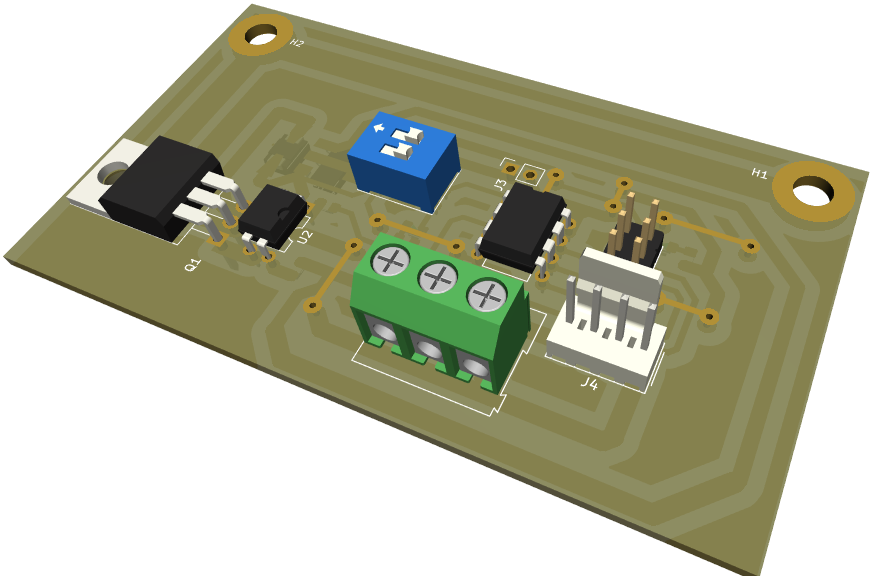
\includegraphics[width=0.8\textwidth,right]{images/halodc_flicker_v0.png}
		\end{minipage}
	\end{figure}

	\raggedright
	
	\section{Firmware Draft}
	
	\begin{minted}[frame=lines,framesep=2mm,fontsize=\footnotesize,bgcolor=LightGray]{c}
#include <avr/io.h>
#include <util/delay.h>

#define FLICK_SLOW 1000
#define FLICK_FAST 200

#define FLICK_MODE_SLOW 0
#define FLICK_MODE_FAST 1

#define FLICK_FN _delay_ms
#define FLICK_MAX_CNT   6

static uint8_t flick_mode, flick_count;

int main(void)
{
	// CONTROL PIN
	DDRB |= 1<<3;
	PORTB &= ~(1<<3);
	
	flick_mode = FLICK_MODE_FAST;
	flick_count = 0;
	
	while (1) {
	  if(flick_mode==FLICK_MODE_FAST) FLICK_FN(FLICK_FAST);
	  else if(flick_mode==FLICK_MODE_SLOW) FLICK_FN(FLICK_SLOW);
		
	  PORTB ^= 1<<3;
	  flick_count++;
		
	  if(flick_count==FLICK_MAX_CNT){
	    if(flick_mode==FLICK_MODE_FAST) flick_mode=FLICK_MODE_SLOW;
		else if(flick_mode==FLICK_MODE_SLOW) flick_mode=FLICK_FAST;
		flick_count=0;
	  }
	}
	return 0;
}
	\end{minted}
	
	\section{Circuit Usage}

	\begin{figure}[h]
		\centering
		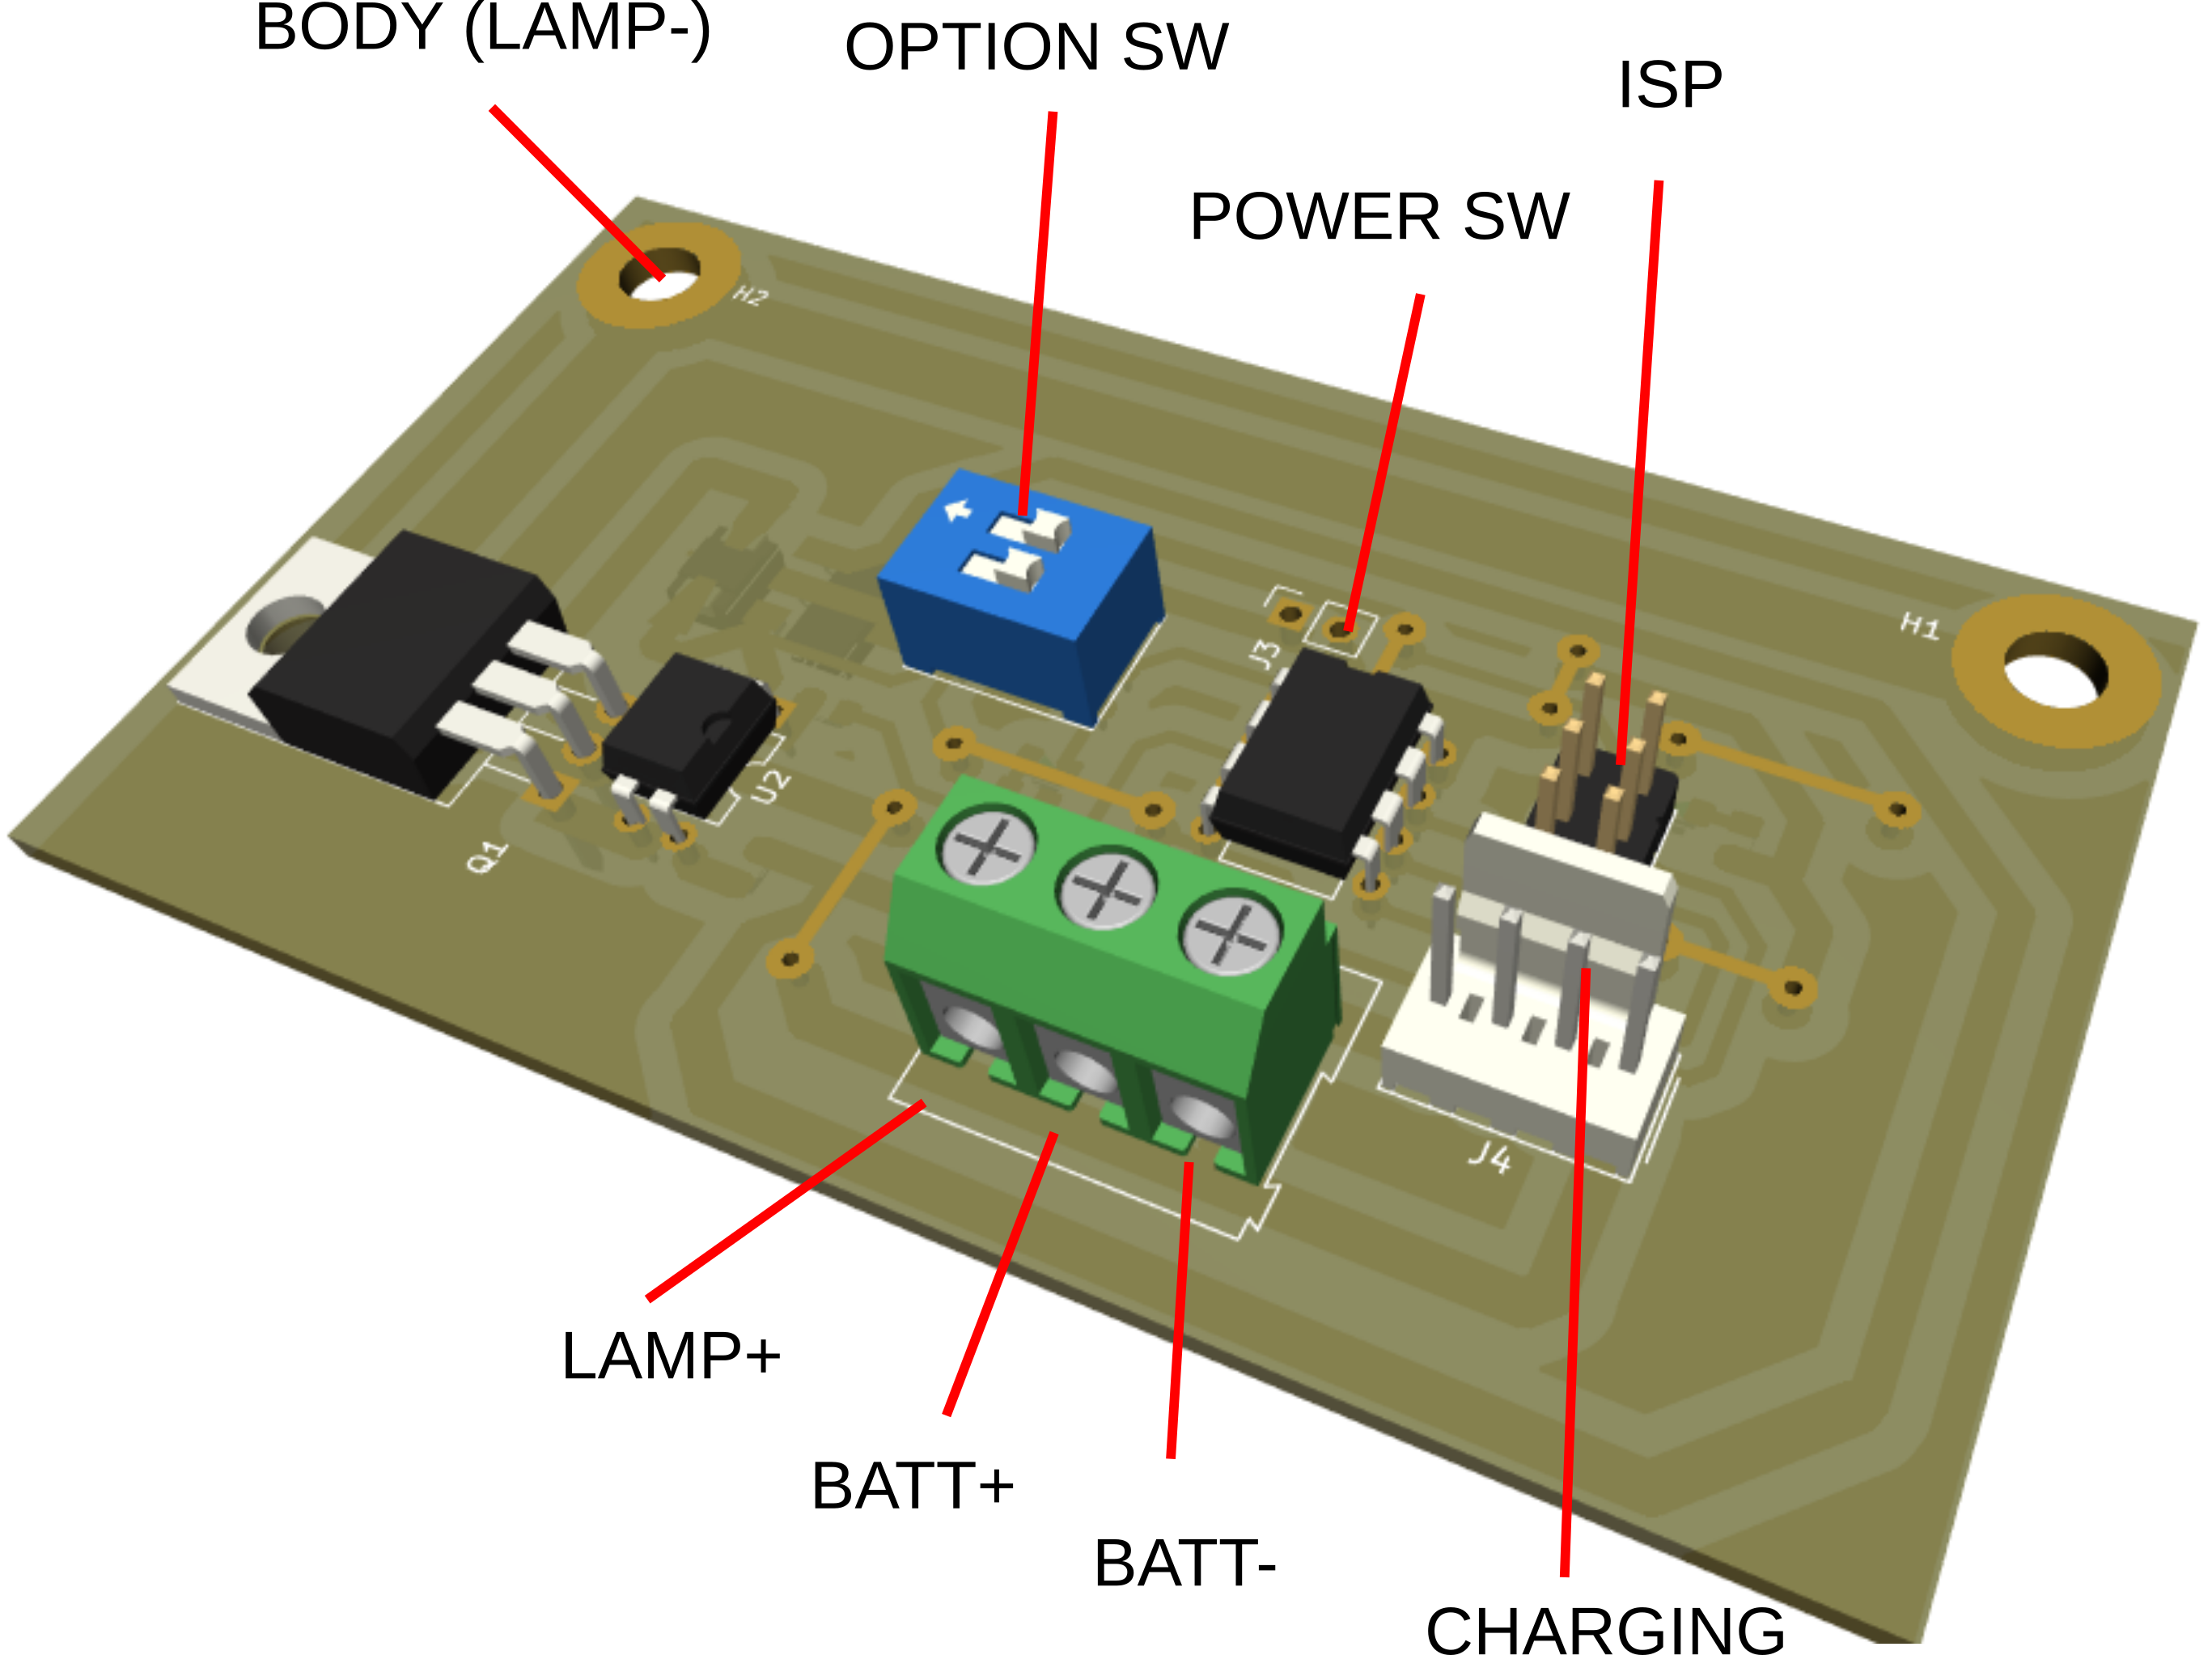
\includegraphics[width=\textwidth]{images/part.png}
		\caption{Circuit Usage}
	\end{figure}
	
	\section{Circuit Design}
	
	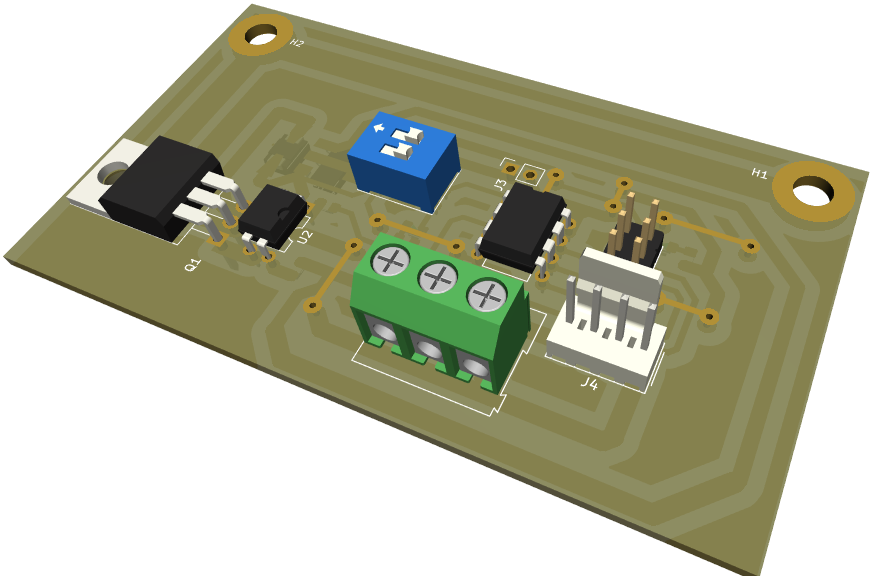
\includepdf[pages=-]{images/halodc_flicker_v0.pdf}
	
	\includepdf[pages=-]{images/halodc_flicker_v0__Assembly.pdf}
	
	\newpage
	\section{Bill of Material}
	
	\textbf{NOTE:} Will be updated following local availability. Soon.
	
	\textbf{NOTE:} Will be updated including PCB assembly tools. Soon.
	
	\begin{table}[!ht]
		\centering
		\begin{tabular}{|l|l|l|l|l|l|l|l|}
			\hline
			Id & Designator & Footprint & Quantity & Designation & Supplier and ref & ~ & ~ \\ \hline
			1 & R2 & R\_0805\_2012Metric\_Pad1.20x1.40mm\_HandSolder & 1 & 10K & ~ & ~ & ~ \\ \hline
			2 & U3 & SOT-223-3\_TabPin2 & 1 & AMS1117-5.0 & ~ & ~ & ~ \\ \hline
			3 & R1,R4,R3 & R\_0805\_2012Metric\_Pad1.20x1.40mm\_HandSolder & 3 & 100 & ~ & ~ & ~ \\ \hline
			4 & U2 & DIP-4\_W7.62mm & 1 & PC817 & ~ & ~ & ~ \\ \hline
			5 & C2,C3,C1 & C\_0805\_2012Metric\_Pad1.18x1.45mm\_HandSolder & 3 & 100nF & ~ & ~ & ~ \\ \hline
			6 & D2 & D\_SMB-SMC\_Universal\_Handsoldering & 1 & D\_Schottky & ~ & ~ & ~ \\ \hline
			7 & U1 & SOIC-8W\_5.3x5.3mm\_P1.27mm & 1 & ATtiny13A-S & ~ & ~ & ~ \\ \hline
			8 & J4 & Molex\_KK-254\_AE-6410-04A\_1x04\_P2.54mm\_Vertical & 1 & CHARGER & ~ & ~ & ~ \\ \hline
			9 & J1 & PinHeader\_2x03\_P2.54mm\_Vertical & 1 & ASP & ~ & ~ & ~ \\ \hline
			10 & H2,H1 & MountingHole\_4.5mm\_Pad & 2 & MountingHole\_Pad & ~ & ~ & ~ \\ \hline
			11 & J2 & TerminalBlock\_Altech\_AK300-3\_P5.00mm & 1 & BATT\_LAMP & ~ & ~ & ~ \\ \hline
			12 & SW1 & SW\_DIP\_SPSTx02\_Slide\_9.78x7.26mm\_W7.62mm\_P2.54mm & 1 & SW\_DIP\_x02 & ~ & ~ & ~ \\ \hline
			13 & Q1 & TO-220-3\_Horizontal\_TabDown & 1 & IRF540N & ~ & ~ & ~ \\ \hline
			14 & D3,D1 & LED\_0805\_2012Metric\_Pad1.15x1.40mm\_HandSolder & 2 & LED & ~ & ~ & ~ \\ \hline
			15 & SW2 & SW\_Tactile\_SPST\_Angled\_PTS645Vx31-2LFS & 1 & SW\_Push & ~ & ~ & ~ \\ \hline
		\end{tabular}
	\end{table}
	
	\section{Shopping}
	
	\subsection{Components}
	
	\begin{table}[!ht]
		\centering
		\begin{tabular}{|l|l|l|l|l|l|l|}
			\hline
			Item & Toko & Kota & Qty & Price & Total & URL \\ \hline
			Dip Switch 2P & Mega Gemilang & Glodok & 2 & IDR 1,800.00 & IDR 3,600.00 & \href{https://www.tokopedia.com/megagemilangglodok/dip-switch-2p}{Tokopedia} \\ \hline
			AMS1117 5V & PCM ElekPusat & Glodok & 3 & IDR 3,000.00 & IDR 9,000.00 & \href{https://www.tokopedia.com/pcmelektronik/ic-ams1117-5v-5}{Tokopedia} \\ \hline
			D SCHOTTKY & PCM ElekPusat & Glodok & 3 & IDR 1,000.00 & IDR 3,000.00 & \href{https://www.tokopedia.com/pcmelektronik/ss310-sma-do-214ac-3a-100v-smd-schottky-rectifier-diode}{Tokopedia} \\ \hline
			Header 1x40 & PCM ElekPusat & Glodok & 2 & IDR 850.00 & IDR 1,700.00 & \href{https://www.tokopedia.com/pcmelektronik/pin-header-male-1x40-single}{Tokopedia} \\ \hline
			IRF540N & PCM ElekPusat & Glodok & 3 & IDR 8,000.00 & IDR 24,000.00 & \href{https://www.tokopedia.com/pcmelektronik/transistor-mosfet-irf-540-irf540n-irf540n}{Tokopedia} \\ \hline
			LED 0805 & PCM ElekPusat & Glodok & 6 & IDR 500.00 & IDR 3,000.00 & \href{https://www.tokopedia.com/pcmelektronik/led-smd-biru-0805}{Tokopedia} \\ \hline
			PC817 & PCM ElekPusat & Glodok & 3 & IDR 750.00 & IDR 2,250.00 & \href{https://www.tokopedia.com/pcmelektronik/pc817-pc-817-optocoupler-pc817-sharp-original-harga-satuan}{Tokopedia} \\ \hline
			Push On & PCM ElekPusat & Glodok & 2 & IDR 3,000.00 & IDR 6,000.00 & \href{https://www.tokopedia.com/pcmelektronik/push-on}{Tokopedia} \\ \hline
			R0805 10K & PCM ElekPusat & Glodok & 3 & IDR 500.00 & IDR 1,500.00 & \href{https://www.tokopedia.com/pcmelektronik/resistor-smd-0805-103-10k-ohm}{Tokopedia} \\ \hline
			R0805 220 & PCM ElekPusat & Glodok & 6 & IDR 500.00 & IDR 3,000.00 & \href{https://www.tokopedia.com/pcmelektronik/resistor-smd-0805-221-220-ohm}{Tokopedia} \\ \hline
			Terminal 3P & PCM ElekPusat & Glodok & 3 & IDR 900.00 & IDR 2,700.00 & \href{https://www.tokopedia.com/pcmelektronik/terminal-pcb-block-screw-3pin-kf301}{Tokopedia} \\ \hline
			ATTiny13a SMD & Tastronik & Bandung & 3 & IDR 13,000.00 & IDR 39,000.00 & \href{https://www.tokopedia.com/tastronik/attiny13a-ssu-smd-attiny-13-attiny13-atmega-avr-marking-tipe-2}{Tokopedia} \\ \hline
		\end{tabular}
	\end{table}
	
	\newpage
	\subsection{PCB}
	
	Estimasi: IDR 152,892.00 (2 pieces) di \href{https://www.tokopedia.com/raftech/jasa-cetak-pcb-general}{Tokopedia}
	
	\begin{figure}[h]
		\centering
		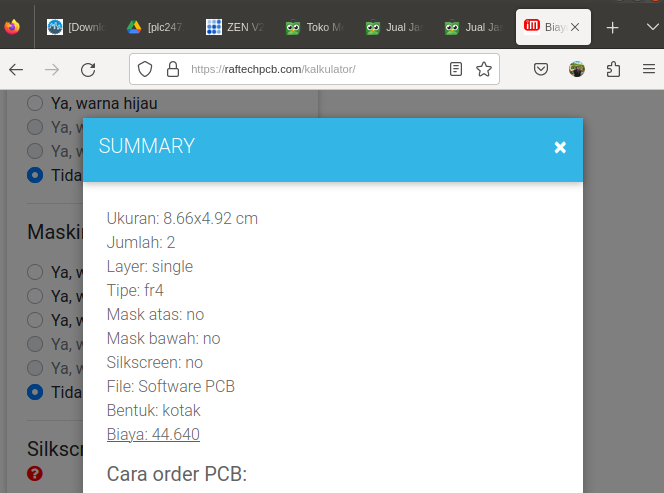
\includegraphics[width=0.6\textwidth]{images/pcb_quotes.png}
		\caption{PCB Quotes}
	\end{figure}
	
	\subsection{Tools}
	
	\begin{table}[!ht]
		\centering
		\begin{tabular}{|l|l|l|l|l|l|l|}
			\hline
			Item & Toko & Kota & Qty & Price & Total & URL \\ \hline
			Solder Dekko 40W & PCM Elek Pusat & Glodok & 1 & IDR 55,000.00 & IDR 55,000.00 & \href{https://www.tokopedia.com/pcmelektronik/soldering-solder-iron-dekko-deko-40w-40-watr}{Tokopedia} \\ \hline
			Pinset Dekko & PCM Elek Pusat & Glodok & 1 & IDR 22,000.00 & IDR 22,000.00 & \href{https://www.tokopedia.com/pcmelektronik/pinset-dekko-tekuk-bagus-ori}{Tokopedia} \\ \hline
			Timah Pancing & PCM Elek Pusat & Glodok & 1 & IDR 22,500.00 & IDR 22,500.00 & \href{https://www.tokopedia.com/pcmelektronik/timah-solder-1-rol-10-meter-merk-pancing}{Tokopedia} \\ \hline
		\end{tabular}
	\end{table}
	
	\subsection{Total}
	
	\begin{table}[!ht]
		\centering
		\begin{tabular}{|l|l|}
			\hline
			Group & Total \\ \hline
			Komponen & IDR 98,750.00 \\ \hline
			PCB & IDR 152,892.00  \\ \hline
			Tools & IDR 99,500.00 \\ \hline
			Ongkir & IDR 50,000.00 \\ \hline
		\end{tabular}
	\end{table}
	
	Estimasi Total: IDR 401,142.00
	
\end{document}
